
\documentclass[a4paper]{article}

\usepackage[english]{babel}
\usepackage[utf8]{inputenc}
\usepackage{graphicx}
\usepackage{float}
\usepackage{url}
\usepackage{amsmath}
\usepackage{algorithm}
\usepackage[noend]{algpseudocode}
\usepackage{tikz}
\usepackage{sudoku}
\usepackage{array}



%Custom commands for logical operators and other pseudocode stuff
\algnewcommand\AND{\textbf{ and }}
\algnewcommand\OR{\textbf{ or }}
\algnewcommand\NOT{\textbf{not}}
\algnewcommand\BREAK{\textbf{break}}
\algnewcommand\RETURN{\textbf{return}}

\author{Rylan Perumal, Tamlin Love, Jia Hao Huo}

\date{\today}

\begin{document}
\begin{titlepage}
	\centering
	

\includegraphics[scale=0.6]{index.png}
	\vspace{0.5cm}
	
\newcommand{\HRule}{\rule{\linewidth}{0.5mm}} 

{\scshape\Large University of Witwatersrand\par}
{\scshape\Large Johannesburg, South Africa\par}
	\vspace{1cm}
	{\huge\bfseries Advanced Analysis of Algorithms Assignment \par}
	\vspace{1cm}
	{\Large\itshape Rylan Perumal, Tamlin Love, Jia Hao Huo\par}
	\vspace{0.5cm}
	{\Large\itshape 1396469, 1438243, 1475365\par}
	\vfill
	
\HRule \\[0.4cm]
{ \huge \bfseries Analysis of the Backtracking Algorithm in the solving of Sudoku problems}\\[0.4cm] 
\HRule \\[1.5cm]

	{\large Semester 2, 2018\par}

\end{titlepage}
\section{Introduction}
Backtracking is a very important family of algorithms used to solve a variety of problems. It operates by incrementally "guessing" a partial solution to a problem. As soon as a partial solution leads to an incorrect solution, the algorithm "backtracks" to an earlier partial solution and attempts other options, much like a depth first search.
\newline
Backtracking algorithms are incredibly powerful tools, as they are guaranteed to find a solution to an appropriate problem, given that the problem is finite and that a solution exists. They are generally much faster than brute force approaches, as they can rule out partial solutions.
\newline
In this project, we will apply the backtracking algorithm to solve Sudoku problems. In a Sudoku problem, an $n^2 \times n^2$ grid is divided into $n^2$ sub-grids of size $n \times n$. Commonly, $n=3$, and thus we consider only this case. Each space in the grid is given a number, to which the following restrictions apply:
\begin{itemize}
    \item A number may not appear more than once in any row
    \item A number may not appear more than once in any column
    \item A number may not appear more than once in any sub-grid
\end{itemize}
\begin{figure}[H]
    \centering
    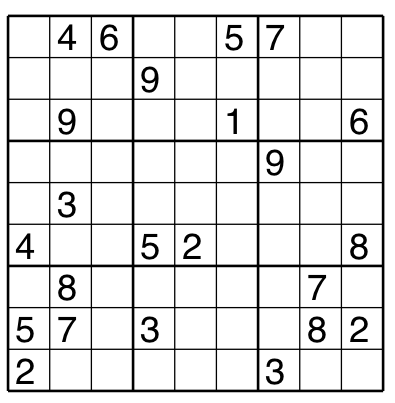
\includegraphics[scale=0.5]{sudoku.png}
    \caption{An example of a Sudoku puzzle, where enough clues are given such that the solution is unique \cite{watanabe_2013}}
    \label{fig:sudokuGridExample}
\end{figure}
We can clearly see that this is the kind of problem in which backtracking algorithms excel. Our strategy is to incrementally fill in the squares, ensuring that the restrictions above are met. If at any stage the algorithm encounters a situation in which no guess is valid, it will backtrack and attempt other guesses.
\section{Theoretical Analysis}
In this analysis, we will compute the algorithm's complexity with respect to $k$, the number of 0 entries (i.e. blank entries) in the initial problem. We keep the size of the grid constant at $9 \times 9$, and thus our complexity will not vary with respect to the size of the grid.
\newline
We will consider stack operations (e.g. \textit{stack.push()} and \textit{stack.pop()}) to be the basic operations. This is equivalent to selecting changes in the state of the grid (i.e. our guesses) as our basic operation.
\newline
We begin by providing a brief pseudocode representation of our implementation of the backtracking algorithm.
\begin{algorithm}[H]
\caption{Backtracking Sudoku Solver}\label{backtrack}
\begin{algorithmic}[1]
\Procedure{Solve}{sudoku}
    \State stack $\gets []$
    \State num $\gets 1$
    \State $i,j \gets 0$
    \While{$\NOT$ isComplete(sudoku)}
        \If{$j \bmod 9 = 0 \AND j \neq 0$}
            \State $i \gets i+1$
            \State $j \gets 0$
        \EndIf
        \State current $\gets$ sudoku[$i$][$j$]
        \If{current.num $=0$}
            \If{checkRCS($i,j$,num,sudoku) $=$ false$\AND$num $<10$}
                \State current.num $\gets$ num
                \State stack.push(current)
                \State num $\gets 0$
                \State $j \gets j+1$
            \Else
                \If{num $>10$}
                    \If{stack.notEmpty()$=$true}
                        \State current $\gets$ stack.pop()
                        \State $i \gets $ current.$i$
                        \State $j \gets $ current.$j$
                        \State num $\gets $ current.num
                        \State current.num $\gets 0$
                    \Else
                        \State $\BREAK$
                    \EndIf
                \EndIf
            \EndIf
        \Else
            \State $j \gets j+1$
            \State num $\gets 0$
        \EndIf
        \State num $\gets$ num$+1$
    \EndWhile
    \State $\RETURN$ sudoku
\EndProcedure
\end{algorithmic}
\end{algorithm}
In the above algorithm, the \textit{isComplete(sudoku)} function checks the grid, \textit{sudoku}, for any 0 entries, returning true if there are no 0's present and false otherwise. The \textit{checkRCS(i,j,num,sudoku)} returns true if \textit{num} occurs in the current row, the current column or the current square. Otherwise, it returns false. Both these functions do not depend on the number of zero entries ($k$) and thus are $\mathcal{O}(1)$. We can therefore safely ignore them for the remainder of this analysis.
\newline
Our first consideration must be of the Best Case. This occurs when our initial guess (for this algorithm, 1) is correct (for $k>9$, we extend this case to encompass other early guesses). In this case, the if-statement on line 11 always evaluates as true when it is reached, and thus the value of \textit{num} never exceeds 1. Since the aforementioned if-statement only executes if \textit{current.num}$=0$, which is only true for $k$ spaces in the grid, the stack operation on line 13 runs only $k$ times, and thus the Best Case complexity is $\mathcal{O}(k)$.
\newline
Conversely, the Worst Case occurs when our final guesses are correct, thus forcing the algorithm to perform maximal backtracking. In this case, the algorithm reduces to a brute force approach. The complexity is thus $\mathcal{O}(9^k)$.
\newline
The Average Case is not trivial to compute theoretically, and is beyond the scope of this paper. We know for sure that the average case has a complexity between $\Omega(k)$ and $\mathcal{O}(9^k)$. We hypothesise that the average case time complexity of the algorithm is $\mathcal{O}(C^k)$ for some $1<C\leq 9$, the average number of guesses per backtrack. We will investigate this hypothesis further through empirical analysis.
\section{Empirical Analysis}
\subsection{Data Processing}
Before we could conduct any meaningful experiments, we required a large data-set of Sudoku problems. We sourced 50 Sudoku problems online, whose solutions exist and are unique \cite{fontaine_2012}. We then augmented the size of our data-set by solving each problem and subsequently "unsolving" then by removing random elements. We started off be removing 1 random element up to removing 64 random elements from each solved puzzle. The reason we removed up to 64 elements is that the minimum number of clues required for the solution of the solved puzzle to be unique is 17 \cite{sudoku_17}. Thus we have generated 3200 new puzzles to be solved.
\newline
\begin{figure}[H]
\centering
 \setlength\sudokusize{4cm}
 \renewcommand\sudokuformat[1]{\sffamily#1}
\begin{sudoku}
|4|8|3|9|2|1|6|5|7|.
|9|6|7|3|4|5|8|2|1|.
|2|5|1|8|7|6|4|9|3|.
|5|4|8|1|3|2|9|7|6|.
|7|2|9|5|6|4|1|3|8|.
|1|3|6|7|9|8|2|4|5|.
|3|7|2|6|8|9|5|1|4|.
|8|1|4|2|5|3|7|6|9|.
|6|9|5|4|1|7|3|8|2|.
\end{sudoku}
\caption{Example unique solution 1}
\end{figure}
\begin{figure}[H]
\centering
 \setlength\sudokusize{4cm}
 \renewcommand\sudokuformat[1]{\sffamily#1}
\begin{sudoku}
|4|8|3|9|2|1|6|5|7|.
|9|6|7|3|4|5|8|2|1|.
|2|5|1|8|7|6|4|9|3|.
|5|4|8|1|3|2|9|7|6|.
|7|2|9|5|6|4|1|3|8|.
|1|3|6|7|9|8|2|4|5|.
|3|7|2|6| |9|5|1|4|.
|8|1|4|2|5|3|7|6|9|.
|6|9|5|4|1|7|3|8|2|.
\end{sudoku}
\caption{Removing 1 value i.e Order 1}
\end{figure}

\begin{figure}[H]
\centering
 \setlength\sudokusize{4cm}
 \renewcommand\sudokuformat[1]{\sffamily#1}
\begin{sudoku}
|4|8| | | | | | |7|.
| | |7| | |5|8|2|1|.
| | |1|8|7| |4| |3|.
| |4| |1| | |9|7| |.
|7|2|9|5|6|4|1| |8|.
|1|3|6|7|9|8|2| |5|.
| | | | | |9|5| | |.
|8|1| |2| |3|7|6|9|.
| |9|5| |1|7|3|8|2|.
\end{sudoku}
\caption{Removing 32 values i.e Order 32}
\end{figure}

\begin{figure}[H]
\centering
 \setlength\sudokusize{4cm}
 \renewcommand\sudokuformat[1]{\sffamily#1}
\begin{sudoku}
|4| | | | | | | | |.
| | | | | | | | |1|.
| | | |8| | | | | |.
| |4| |1| | | | | |.
| | | |5|6|4|1| |8|.
|1| |6| | | | | | |.
| | | | | | | | | |.
| | | | | | | |6| |.
| |9|5| | | | |8|2|.
\end{sudoku}
\caption{Removing 64 values i.e Order 64}
\end{figure}


\newpage
\subsection{Experiment}
Graphing the execution time of the algorithm against the number of zero entries ($k$), we arrive at the following.
\begin{figure}[H]
    \centering
    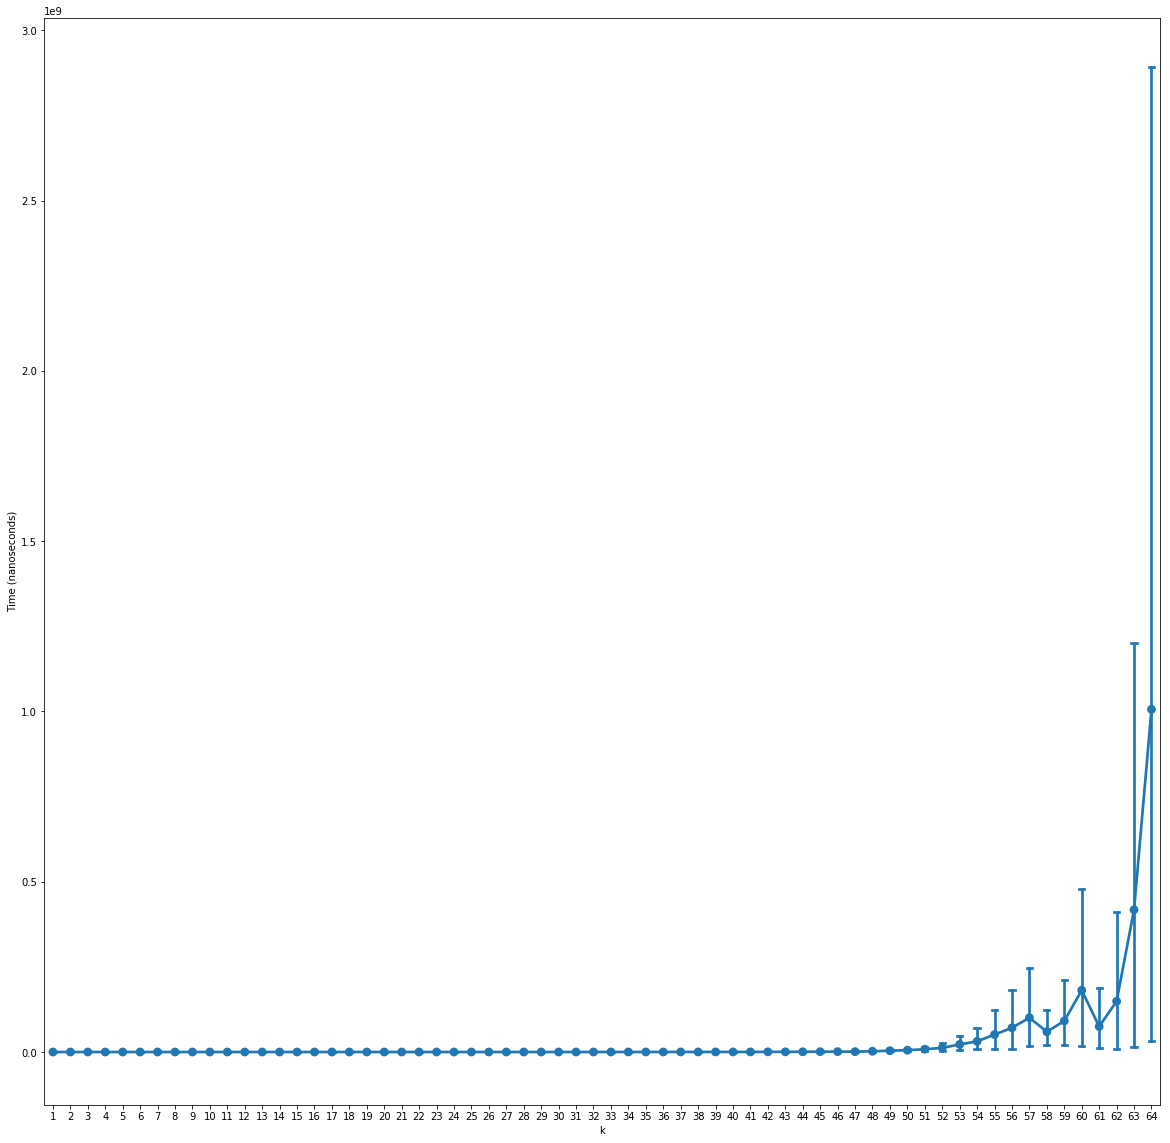
\includegraphics[scale=0.3]{experiment1.png}
    \caption{Time (in nanoseconds) vs. Number of 0 entries ($k$)}
    \label{fig:experiment1}
\end{figure}
The following statistical figures relate to this data-set
\begin{table}[H]
    \centering
    \begin{tabular}{|l|l|}
        \hline
        Count                   & 3200                  \\ \hline
        Mean                    &  0.03589 seconds      \\ \hline
        Standard Deviation      &  0.90084              \\ \hline
        Minimum                 &  0.00000119 seconds  \\ \hline
        25\%                    &  0.00003279 seconds  \\ \hline
        50\%                    &  0.00008533 seconds  \\ \hline
        75\%                    &  0.00054657 seconds  \\ \hline
        Maximum                 &  45.85793 seconds     \\ \hline
    \end{tabular}
\end{table}
\newpage
Graphing, instead, the number of stack operations against $k$, we arrive at the following figure.
\begin{figure}[H]
    \centering
    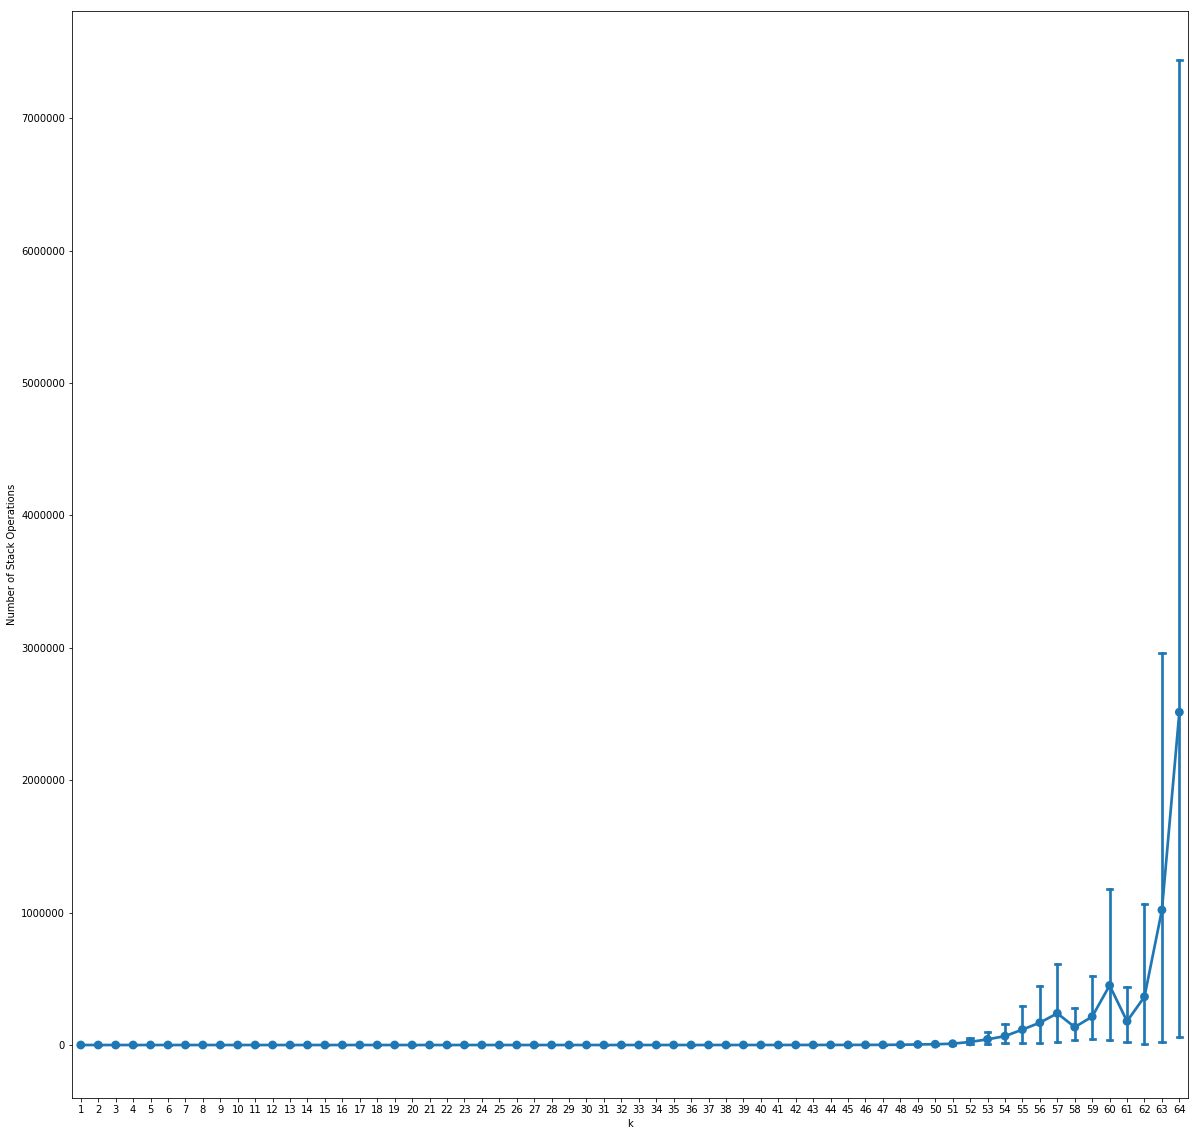
\includegraphics[scale=0.3]{experiment2.png}
    \caption{Number of stack operations vs. Number of 0 entries ($k$)}
    \label{fig:experiment2}
\end{figure}
The following statistical figures relate to this data-set
\begin{table}[H]
    \centering
    \begin{tabular}{|l|l|}
        \hline
        Count                   & 3200                      \\ \hline
        Mean                    &  86941.75 operations      \\ \hline
        Standard Deviation      &  2260370                  \\ \hline
        Minimum                 &  1 operation              \\ \hline
        25\%                    &  17 operations            \\ \hline
        50\%                    &  53 operations            \\ \hline
        75\%                    &  477.5 operations         \\ \hline
        Maximum                 &  115201800 operations     \\ \hline
    \end{tabular}
\end{table}
\newpage
\section{Discussion}
Our first remark when comparing figures \ref{fig:experiment1} and \ref{fig:experiment2} is that they have incredibly similar shapes. Thus the number of stack operations closely correlates with the time taken for the algorithm to execute. This indicates that our choice of basic operation at the beginning of Section 2 was pertinent.
\newline
Our second observation is to note that the shape of these graphs match up closely with the shapes of functions of the form $C^x$ (see figure \ref{fig:nineToTheK}), for some constant $C$. Our algorithm is bounded above by the worst case, $\mathcal{O}(9^k)$. It therefore makes intuitive sense that the average case of our algorithm would be some $\mathcal{O}(C^k)$ for $1<C\leq9$, supporting our theoretical analysis.
\begin{figure}[H]
    \centering
    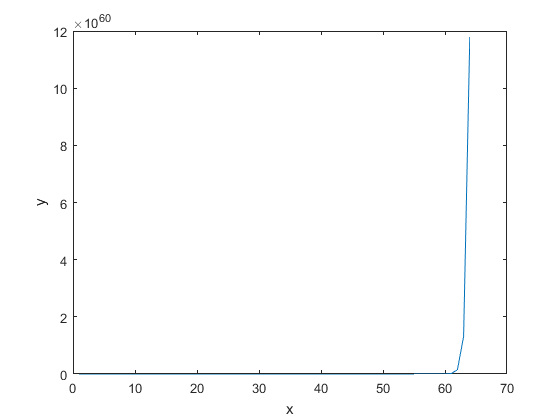
\includegraphics[scale=0.6]{nineToTheK.png}
    \caption{Graph of $y=9^x$}
    \label{fig:nineToTheK}
\end{figure}
Unfortunately, however, the difficulty of a Sudoku problem can have massive effects on the results for large $k$ (See the vertical variation for larger $k$ values in figures \ref{fig:experiment1} and \ref{fig:experiment2}). Quantifying the difficulty is not trivial, and depends on one's definition \cite{watanabe_2013}. Nevertheless, if one considers mean values for each $k$, then for large data-sets the difficulties of the individual problems should average each other out. In that case, our discussion above remains valid.
\section{Conclusion}
From our theoretical and empirical analysis, we conclude that the average complexity of our backtracking Sudoku-solving algorithm is $\mathcal{O}(C^k)$ where $1 < C \leq 9$. 
\newline
 Further experimentation is needed to determine the value of $C$.
 \newpage
\bibliographystyle{apalike}
\bibliography{mybib}
\end{document} 

%http://www.sudokuessentials.com/create-sudoku.html \\
%https://www.technologyreview.com/s/426554/mathematicians-solve-minimum-sudoku-problem/ 
